\section{Projektidee und Konzept}\label{sec:projektidee-und-konzept}

Dieses Kapitel beschreibt die Motivation des Studierendenteams hinter dem Projekt in~\ref{subsec:motivation}.
Darauf folgend werden die Ergebnisse einer Umfrage präsentiert, die die Idee einer universellen Plattform zur Dokumentation und Verwaltung von Sammlungen unterstützt, wie in~\ref{subsec:umfrage} beschrieben.

\subsection{Motivation}\label{subsec:motivation}


Das Sammeln von Gegenständen ist eine Leidenschaft, die uns als Studententeam verbindet.
Von LEGO-Sets und Sammelfiguren bis hin zu Videospielen und Parfüms, egal ob aus Wertinteresse oder Selbstverwirklichungsgründen, jedes Mitglied sammelt.
Trotz dessen, dass es so viele verschiedene Sammelgegenstände und Kategorien gibt, verbindet diese Eigenschaft erstaunlich viele Menschen.
Allerdings kennen wir auch die Herausforderungen: Die Pflege mehrerer Sammlungen erfordert Zeit und Organisation.
Nach Diskussion bezüglich, was wir für die Sammlungsdokumentation benutzen, fiel dem Team schnell die Unmenge an verschiedenen speziellen Plattformen auf. \par
Obwohl es viele Plattformen zur Verwaltung einzelner Sammlungen gibt, fehlt bisher eine universelle Lösung, die es uns ermöglicht, all unsere Sammelgegenstände an einem Ort zu digitalisieren und zu organisieren.
Genau das möchten wir mit unserem Praxisprojekt ändern.
Unsere Webseite namens Collectiqo soll vorgefertigte und anpassbare Vorlagen bieten, um Sammlungen jeglicher Art zu dokumentieren und zu präsentieren.
So können wir den Pflegeaufwand reduzieren und unsere Leidenschaft noch besser genießen.


\subsection{Umfrage}\label{subsec:umfrage}

Um Anforderungen an das Projekt zu definieren und die Plattform bestmöglich zu differenzieren, wurde eine Umfrage erstellt.
Diese Umfrage sollte die Motivation für die Durchführung des Projekts erweitern, über das persönliche Interesse der Teammitglieder hinaus.
Teilgenommen an der Umfrage haben 20 Personen, wobei das Studierendenteam selbst nicht daran teilgenommen hat.
Es wurden Fragen bezüglich Sammeln als Eigenschaft, Art der Sammlungen, der Dokumentation und Interesse an einer universellen Plattform gestellt, deren Ergebnisse im Folgenden präsentiert werden.

Die ersten Fragen befassen sich damit, ob die Befragten Sammler sind und wie viele Sammlungen sie besitzen.
Abbildung~\ref{fig:forms_result_01} zeigt, dass 90~\% der Befragten mindestens eine Sammlung besitzen.
Wie Abbildung~\ref{fig:forms_result_02} darstellt, besitzen 66,7~\% sogar mehrere.

\begin{figure}[h]
    \centering
    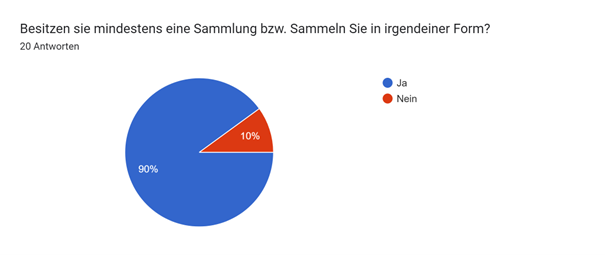
\includegraphics[width=0.86\textwidth]{FORMS_01}
    \caption{Ergebnis der Umfrage: Frage 1}
    \label{fig:forms_result_01}
\end{figure}

\newpage
\begin{figure}[h]
    \centering
    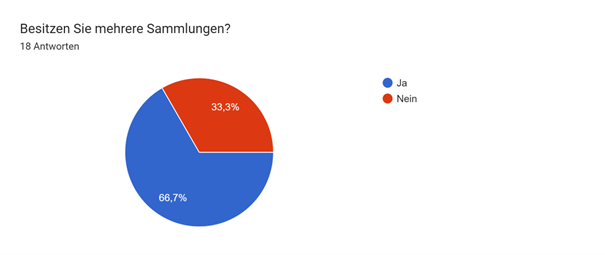
\includegraphics[width=0.86\textwidth]{FORMS_02}
    \caption{Ergebnis der Umfrage: Frage 2}
    \label{fig:forms_result_02}
\end{figure}

Die Motivation hinter dem Sammeln ist vielfältig, wie sich in~\ref{fig:forms_result_03} zeigt: 55~\% der Sammler schätzen den persönlichen Wert ihrer Sammlung, 50~\% betrachten sie als Geldanlage, und ebenso viele sammeln aus Leidenschaft.
Weitere 40~\% sammeln aus dekorativen Gründen, während 5~\% ein historisches Interesse an ihren Sammlungen haben.

Bei der Dokumentation ihrer Sammlungen verwenden 55~\% der Befragten ein Medium, während 45~\% darauf verzichten.
Unter denjenigen, die ein Medium zur Dokumentation nutzen, bevorzugen 44,4~\% ein Buch, 22,2~\% setzen auf Excel-Tabellen oder ähnliche Programme, und 11,1~\% nutzen Online-Plattformen.
Einzelne Personen kombinieren auch verschiedene Medien, etwa Buch und Excel (11,1~\%) oder Excel und Datenbanken (11,1~\%).
Visualisierungen dieser Ergebnisse finden sich in Abbildungen~\ref{fig:forms_result_04} und~\ref{fig:forms_result_05}.

\newpage

\begin{figure}[h!]
    \centering
    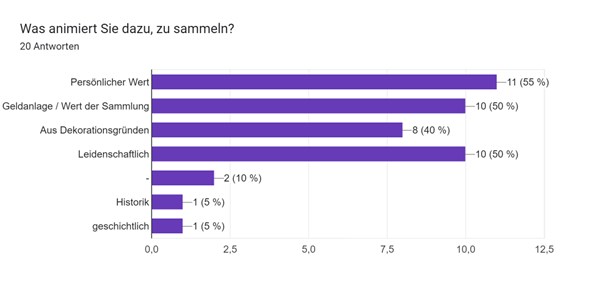
\includegraphics[width=0.86\textwidth]{FORMS_03}
    \caption{Ergebnis der Umfrage: Frage 3}
    \label{fig:forms_result_03}
\end{figure}

\begin{figure}[h!]
    \centering
    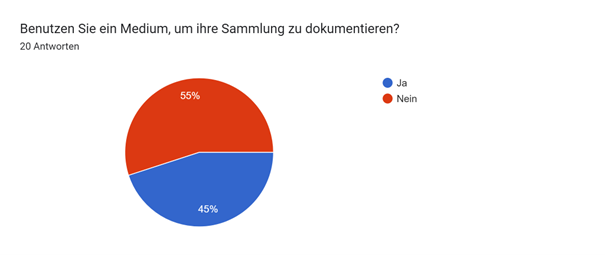
\includegraphics[width=0.86\textwidth]{FORMS_04}
    \caption{Ergebnis der Umfrage: Frage 4}
    \label{fig:forms_result_04}
\end{figure}
\begin{figure}[h!]
    \centering
    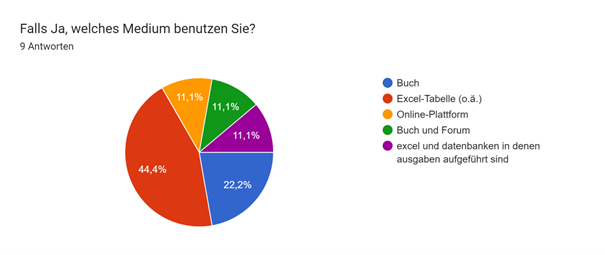
\includegraphics[width=0.86\textwidth]{FORMS_05}
    \caption{Ergebnis der Umfrage: Frage 5}
    \label{fig:forms_result_05}
\end{figure}

Die Idee einer universellen Plattform zur Dokumentation und Verwaltung von Sammlungen wird von den Befragten unterschiedlich bewertet.
Insgesamt finden 55~\% der Sammler die Idee nützlich bis äußerst nützlich, während 40~\% eine neutrale Meinung vertreten.
Letztlich lehnen 5~\% die Plattform vollständig ab, dies steht allerdings in Korrelation mit der Abneigung vom Sammeln aus Frage 1.

Die Ergebnisse in Abbildung~\ref{fig:forms_result_06} zeigen, dass eine universelle Sammlerplattform durchaus auf Interesse stoßen könnte.
Insbesondere die Tatsache, dass ein großer Teil der Sammler bereits Medien zur Dokumentation nutzt und viele Sammler ihre Sammlungen als wertvoll oder leidenschaftlich betrachten, spricht für die Entwicklung einer solchen Plattform.

\begin{figure}[h!]
    \centering
    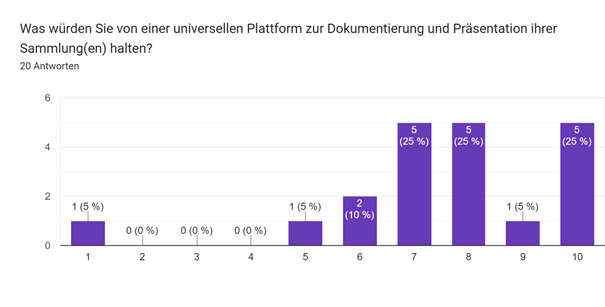
\includegraphics[width=0.86\textwidth]{FORMS_06}
    \caption{Ergebnis der Umfrage: Frage 6}
    \label{fig:forms_result_06}
\end{figure}

